\section{Solutions} \label{sec:solution}

under harsh ringing when the aformentioned equilibrium existence and stability condition does not hold, we show three compensation techniques which stablize the converter and optimize the performance.

\subsection{Analog Comparator Overdrive Propagation Delay}

A new comparator model considering the overdrive propagation delay
The real comparator has a delay from the input edge to output edge (TI Comp Delay). The delay time is actually variable with respect to the input overdrive, which is called overdrive-propagation delay as shown in Fig\;\ref{fig:copd1} and \ref{fig:copd2}. In high-frequency power converter application, it is not accurate enough to just mode the comparator as an ideal comparator. To take the variable delay into consideration, we show the following variable delay comparator model: We start with the physical model of a comparator is in Fig\;\ref{fig:physicalmodel}. It contains a differential input stage and a multi-stage common-source amplifier output. The load, which is usually the next stage CMOS logic integrated circuit, can be simplified as a capacitor. 
\begin{figure}
\begin{minipage}{0.32\textwidth}
    \centering
    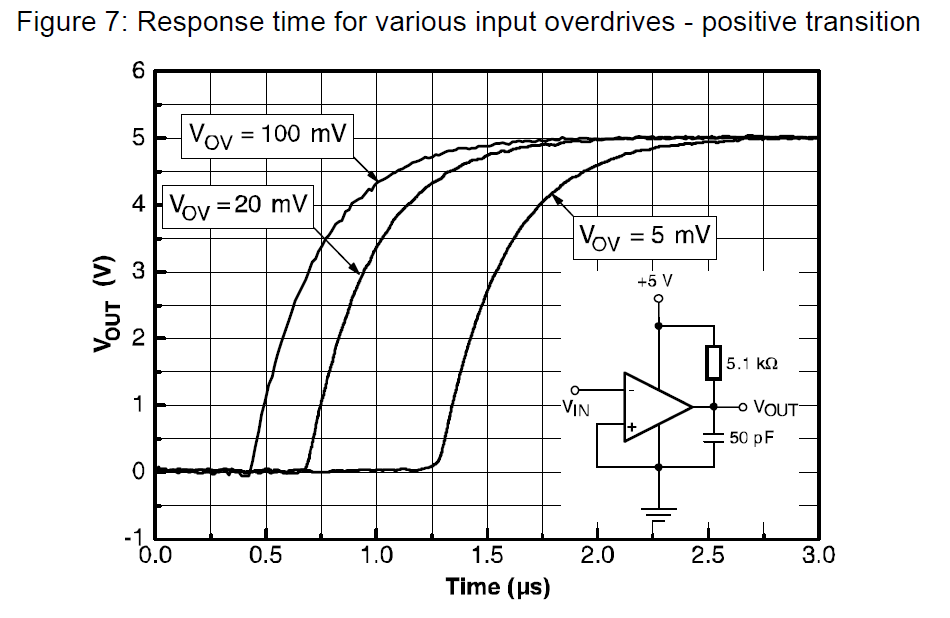
\includegraphics[width=\textwidth]{Figure/section3/copd/copd1.png}
    \caption{ \label{fig:copd1} Comparator Response time various input overdrives.}
\end{minipage}
~
\begin{minipage}{0.32\textwidth}
    \centering
    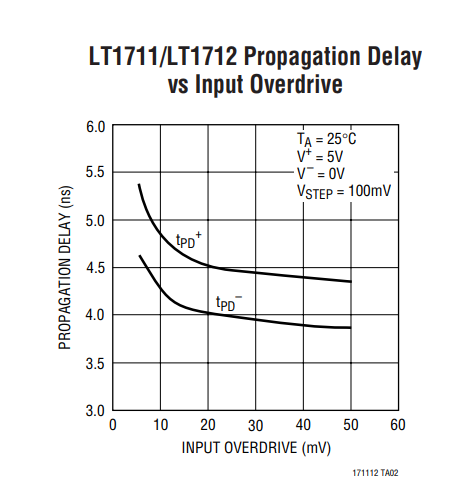
\includegraphics[width=\textwidth]{Figure/section3/copd/copd2.png}
  \caption{  \label{fig:copd2} Comparator Response time various input overdrives(2).}
\end{minipage}
~
\begin{minipage}{0.32\textwidth}
    \centering
    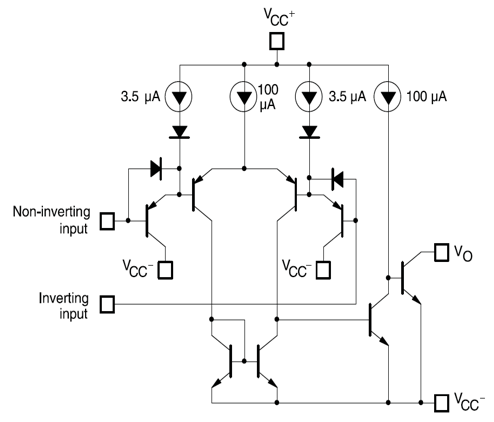
\includegraphics[width=\textwidth]{Figure/section3/copd/physicalmodelcomp.PNG}
    \caption{\label{fig:physicalmodel} Simplified physical model of a comparator.}
\end{minipage}
\end{figure}
To trade-off the balance of model accuracy and analysis complexity, we do reasonable simplification on the comparators system in .Although the large signal gain of the input differential pair is the tanh function of the input overdrive voltage, we use a linear equivalent gain k to approximate the relationship, namely $I_{\text{out}} = k(V_{+} - V_{-})$. We use an integrator block to model the process that output current charges the capacitive load. Then the $V_{\text{th}}$ and an ideal comparator is used to model the process that the following stage is triggered after its input voltage is over the 0.5\,V threshold. 

The simplified model, which we named ''integrator-threshold`` model, proves to capture the main dynamics of the non-ideal comparators by our simulation comparison with the real variable overdrive propagation delay from (LM 193 DS). Fig.3 is the propagation delay from comparator LT1711 datasheet. 
Fig.4 Simulated Overdrive-propagation delay plot using parameters $k = , V_{\text{th}}$. It looks in the similar shape as the simulation result using the following parameters.


The overdrive propagation delay smooths the current command to actual current function $\mathcal{T}$ and improves the stability of the inner current loop.

\begin{figure}
\begin{minipage}{0.32\textwidth}
    \centering
    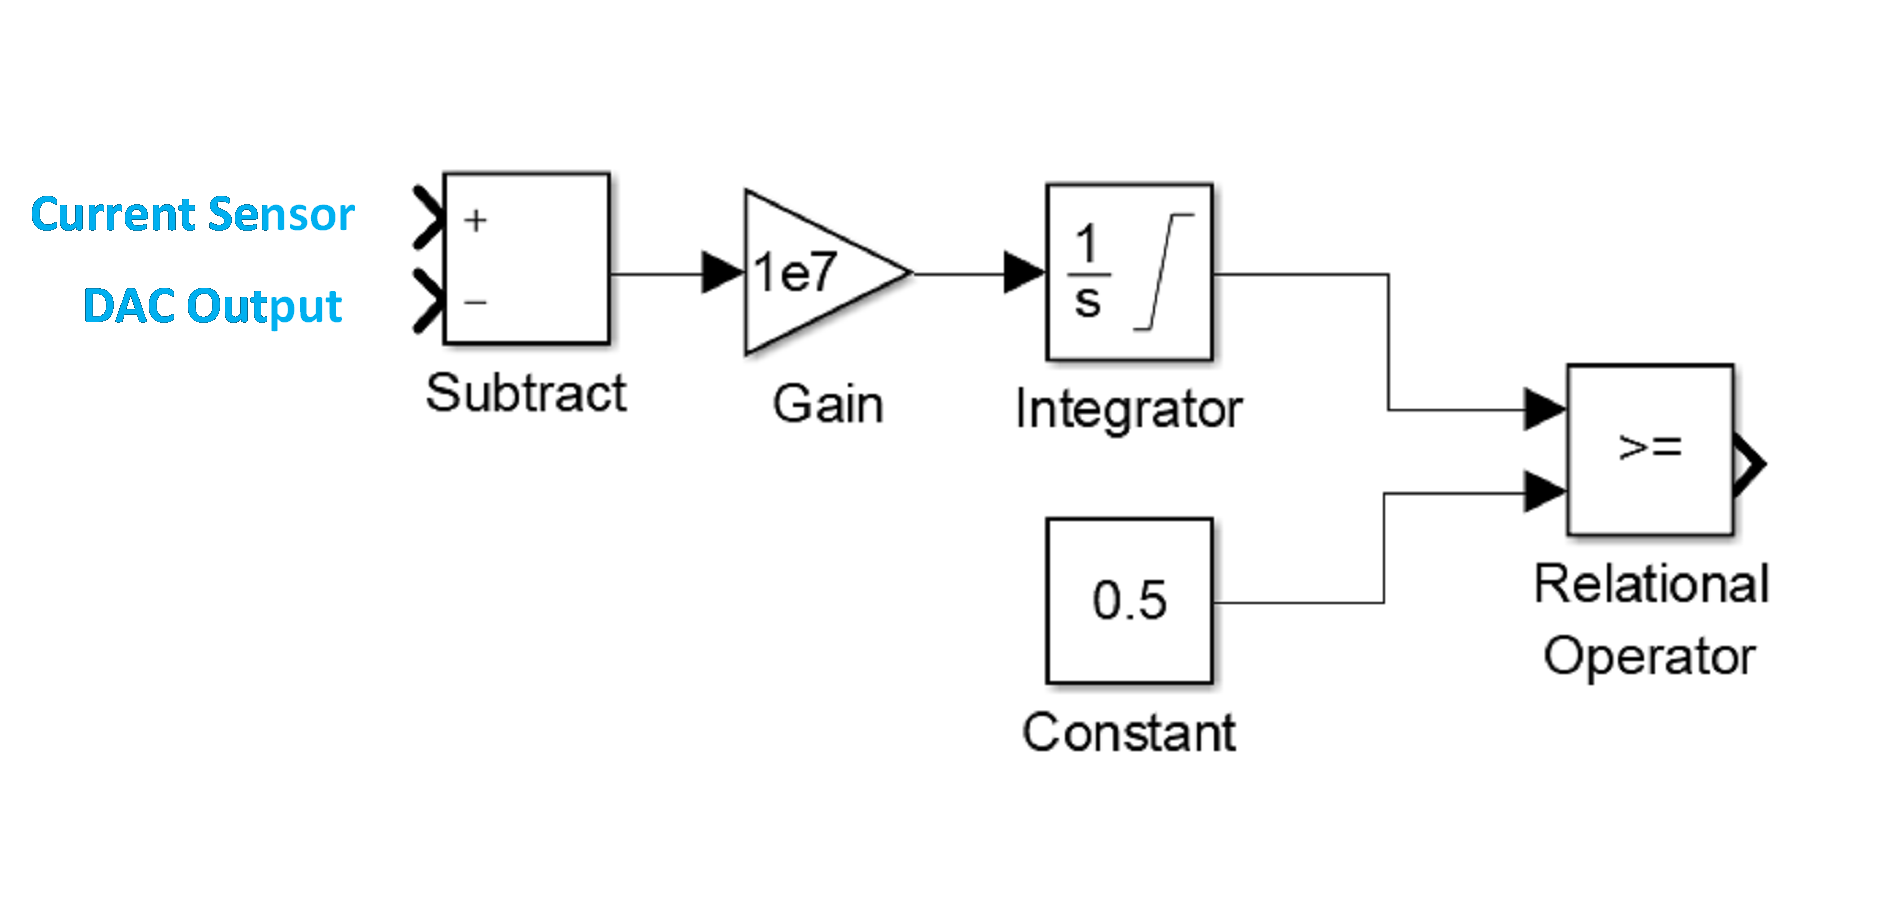
\includegraphics[width=\textwidth]{Figure/section3/copd/mathmodelcomp}
    \caption{ \label{fig:copd1}Simplified mathematic model of a comparator.png}
\end{minipage}
~
\begin{minipage}{0.32\textwidth}
    \centering
    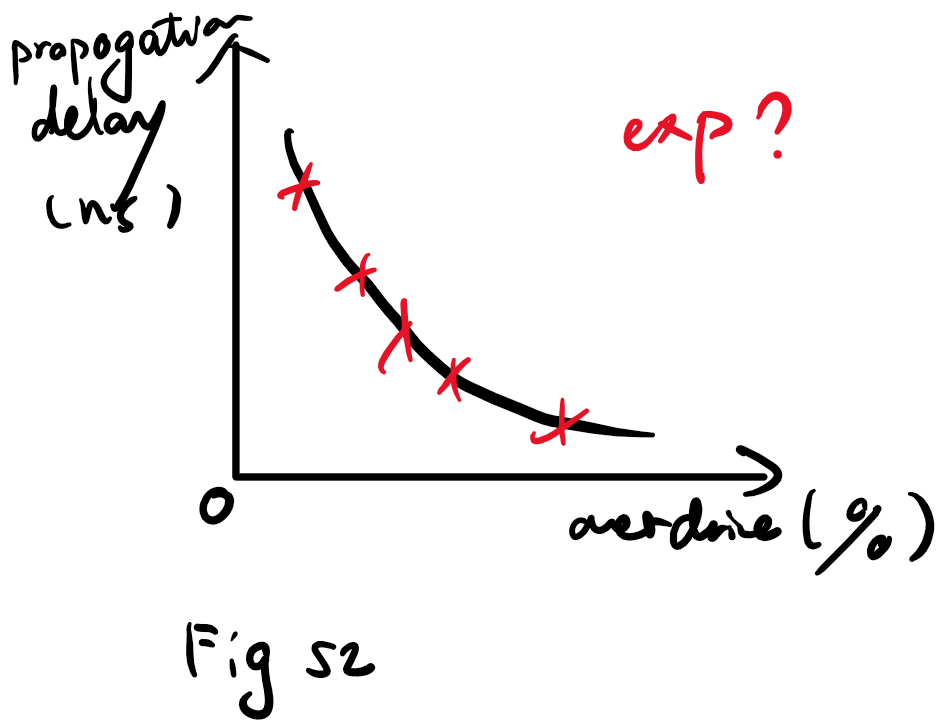
\includegraphics[width=\textwidth]{Figure/section3/copd/simumodelcomp}
  \caption{\label{fig:copd2}Simulated propagation delay using the simplified model of a comparator.}
\end{minipage}
\end{figure}

Fig compares the function $\mathcal{T}$ with and without the overdrive propagation delay. The error gain is a good representative of the overdrive propagation delay. We note that with the increase of the error gain, $\lambda(U\!E)$ decreases. We define the minimum error gain $G_{\text{min}}$ as the error gain which makes $U\!E$ be a zero measurable set. For all $G > G_{\text{min}}$, T is an onto mapping. The algorithm to find out the $G_{\text{min}}$, the minimum gain which make the equilibrium existence condition hold can be found in appendix.

The integrator and threshold mechanism follows
\begin{align} \label{IT}
\int_{t_c}^{t_{\text{on}}} \left(i_p[n-1] - m_2t_{\text{off}} + m_1 t + f(t) - i_c [n] \right) dt = k.
\end{align}
where $k \triangleq V_{\text{th}}/G$ and the crossing time $t_c[n]$ is defined as the solution of equation
\begin{align} \label{DTC}
 m_1 x + f(x)  = i_c [n] - i_p[n-1] + m_2t_{\text{off}}.
\end{align}
We assume the crossing time $t_c[n]$ at the equilibrium is $T_c$.
% Solve the integration in (\ref{IT}),
% \begin{align} \label{IT2}
% &(i_p[n-1] - m_2t_{\text{off}} - i_c [n]) (t_{\text{on}}[n] - t_c[n])  \nonumber \\
% &+ \frac{1}{2}m_1 (t^2_{\text{on}}[n] - t^2_c[n]) + \int_{t_c[n]}^{t_{\text{on}}[n]} f(t) \; dt  = \frac{V_{\text{th}}}{k}.
% \end{align}
Linearize (\ref{IT}):
\begin{align} \label{IT3}
(I_p - m_2t_{\text{off}} - I_c) (\tilde t_{\text{on}}[n] - \tilde t_c[n])  
+(\tilde i_p[n-1] - \tilde i_c [n]) (T_{\text{on}} - T_c)  \nonumber \\
+ m_1 (T_{\text{on}} \tilde t_{\text{on}}[n] - T_c \tilde t_c[n]) +  f(T_{\text{on}}) \tilde t_{\text{on}}[n] - f(T_c) \tilde t_c[n]  = 0.
\end{align}
Substitute (\ref{DTC}) into (\ref{IT3}):
\begin{align} \label{IT4}
(f(T_{\text{on}})-f(T_{c})+m_1(T_{\text{on}}-T_{c}))\tilde{t}_{\text{on}}[n] \nonumber \\
+(\tilde i_p[n-1] - \tilde i_c [n]) (T_{\text{on}} - T_c) =0.
\end{align}
From (\ref{IT4}) and (\ref{ID1}), the small signal model of inner current loop under this compensator is (\ref{iltf1}) with 
\begin{align} \label{S2}
s = m_1 + \frac{f(T_{\text{on}}) - f(T_c)}{T_{\text{on}} - T_c}.
\end{align}
So integrator plus threshold does not help interference function with a fixed slope at all, but it can help with the periodic interference function.
% We assume $f$ is a periodic signal with bounded amplitude $[A_{\text{min}},A_{\text{max}}]$.

Then we want to find the relationship between $T_{\text{on}}$ and $T_c$.
In steady state, 
\begin{align} \label{IT6}
\int_{T_c}^{T_{\text{on}}} \left(I_p - m_2t_{\text{off}} + m_1 t + f(t) - I_c \right) dt = \frac{V_{\text{th}}}{k}.
\end{align}
Solve the integration in (\ref{IT6}),
\begin{align} \label{IT7}
&(I_p - m_2t_{\text{off}} - I_c) (T_{\text{on}} - T_c)  \nonumber \\
&+ \frac{1}{2}m_1 (T^2_{\text{on}} -  T^2_c) + \int_{T_c}^{T_{\text{on}}} f(t) dt  = \frac{V_{\text{th}}}{k}.
\end{align}
Substitute (\ref{DTC}) into (\ref{IT7}):
\begin{align} \label{IT8}
\frac{1}{2}m_1 (T_{\text{on}} - T_c)^2 - f(T_{\text{c}})(T_{\text{on}} - T_c) + \int_{T_c}^{T_{\text{on}}} f(t)\; dt  = \frac{V_{\text{th}}}{k}.
\end{align}
Define this variable delay time $t_d \triangleq T_{\text{on}} - T_c $. From (\ref{sinint}) and (\ref{IT8}),
\begin{align}
t_d = \frac{f(T_{\text{c}})}{m_1} + \sqrt{\left(\frac{f(T_{\text{c}})}{m_1}\right)^2+\frac{2}{m_1}\left(\frac{V_{\text{th}}}{k}-\int f dt \right)}
\end{align}
Because $f$ is a periodic signal, its integral over time is bounded by $[S_{\text{min}}, S_{\text{max}}]$. For example, if we assume $f(t) = A \text{sin}(2\pi f t)$, then 
\begin{align} \label{sinint}
- \frac{A}{\pi f } \leq  \int f dt \leq \frac{A}{\pi f }
\end{align}
We define the upper and lower bound of $t_d$ as $t_u$ and $t_l$
\begin{align}
t_u (f(T_{\text{c}}))= \frac{f(T_{\text{c}})}{m_1} + \sqrt{\left(\frac{f(T_{\text{c}})}{m_1}\right)^2+\frac{2}{m_1}\left(\frac{V_{\text{th}}}{k}-S_{\text{min}} \right)} \nonumber \\
t_l (f(T_{\text{c}}))= \frac{f(T_{\text{c}})}{m_1} + \sqrt{\left(\frac{f(T_{\text{c}})}{m_1}\right)^2+\frac{2}{m_1}\left(\frac{V_{\text{th}}}{k}-S_{\text{max}} \right)}
\end{align}
We notice that both $t_u$ and $t_l$ are monotonically decreasing with $f(T_{\text{c}})$.\\
From (\ref{S2}), the system is stable as long as we design $t_d$ to satisfy the following equation for all $f(T_{\text{c}})$ 
\begin{align} \label{CT1}
m_1 + \frac{A_{\text{min}}-f(T_{\text{c}})}{t_l(f(T_{\text{c}}))} > \frac{m_1}{2}
\end{align}
Besides, we have to impose the following for all $f(T_{\text{c}})$.
\begin{align} \label{CT2}
t_u(f(T_{\text{c}})) \leq T_{\text{on}}
\end{align}
From constraints (\ref{CT1}) and (\ref{CT2}), we can have the $k$ we are supposed to design. Constraint (\ref{CT1}) determines the higher bound of $k_{\text{max}}$ and constraint (\ref{CT2}) determines the lower bound of $k_{\text{min}}$.
Hence, we can get the expression of $k_{\text{min}}$ from the following,
\begin{align}
t_{u_{\text{max}}} = t_u(A_{\text{min}}) = T_{\text{on}}
\end{align}
Then, the expression of minimum $t_l$ is from the following
\begin{align}
t_{l_{\text{min}}}= \frac{A_{\text{min}}}{m_1} + \sqrt{\left(\frac{A_{\text{min}}}{m_1}\right)^2 + \frac{2}{m_1}\left(\frac{V_{\text{th}}}{k}-S_{\text{max}} \right)}
\end{align}

Then the location of the pole can be bounded by
\begin{align} \label{SC21}
a^i_{1_{\text{min}}} =  1 - \frac{1}{1 + \frac{A_{\text{min}}-A_{\text{max}}}{m_1t_{l_{\text{min}}}}} \le a^i_1 \le a^i_{1_{\text{max}}} = 1 - \frac{1}{1 + \frac{A_{\text{max}}-A_{\text{min}}}{m_1t_{l_{\text{min}}}}}
\end{align}


